% ==============================================================================
% APPENDIX
% ==============================================================================
\appendix
\section{Appendix}

\begin{frame}{Appendix: System Modeling}
    \framesubtitle{Linear Model: Least Square Method}
    \begin{columns}[T]
        \begin{column}{0.52\textwidth}

            \begin{block}{Model equations}
                \begin{align*}
                    y_k(t+1)
                        &= a\,y_k(t) + b\,u_k(t) + c \\
                        &= \boldsymbol{\varphi}_k^{\mathsf T}
                           \boldsymbol{\theta}.
                \end{align*}
                \[
                    \boldsymbol{\varphi}_k^{\mathsf T} =
                    \begin{bmatrix} y_k(t) & u_k(t) & 1 \end{bmatrix}
                    \qquad
                    \boldsymbol{\theta} =
                    \begin{bmatrix} a & b & c \end{bmatrix}^{\mathsf T}.
                \]

                The least-squares estimate is
                \begin{equation*}
                    \boldsymbol{\theta}^{\star}
                        =
                        \left(\boldsymbol{\Phi}^{\mathsf T}
                        \boldsymbol{\Phi}\right)^{-1}
                        \boldsymbol{\Phi}^{\mathsf T}\boldsymbol{Y}.
                \end{equation*}
            \end{block}
        \end{column}

        \begin{column}{0.48\textwidth}
            \centering

            \vspace{0.15cm}

            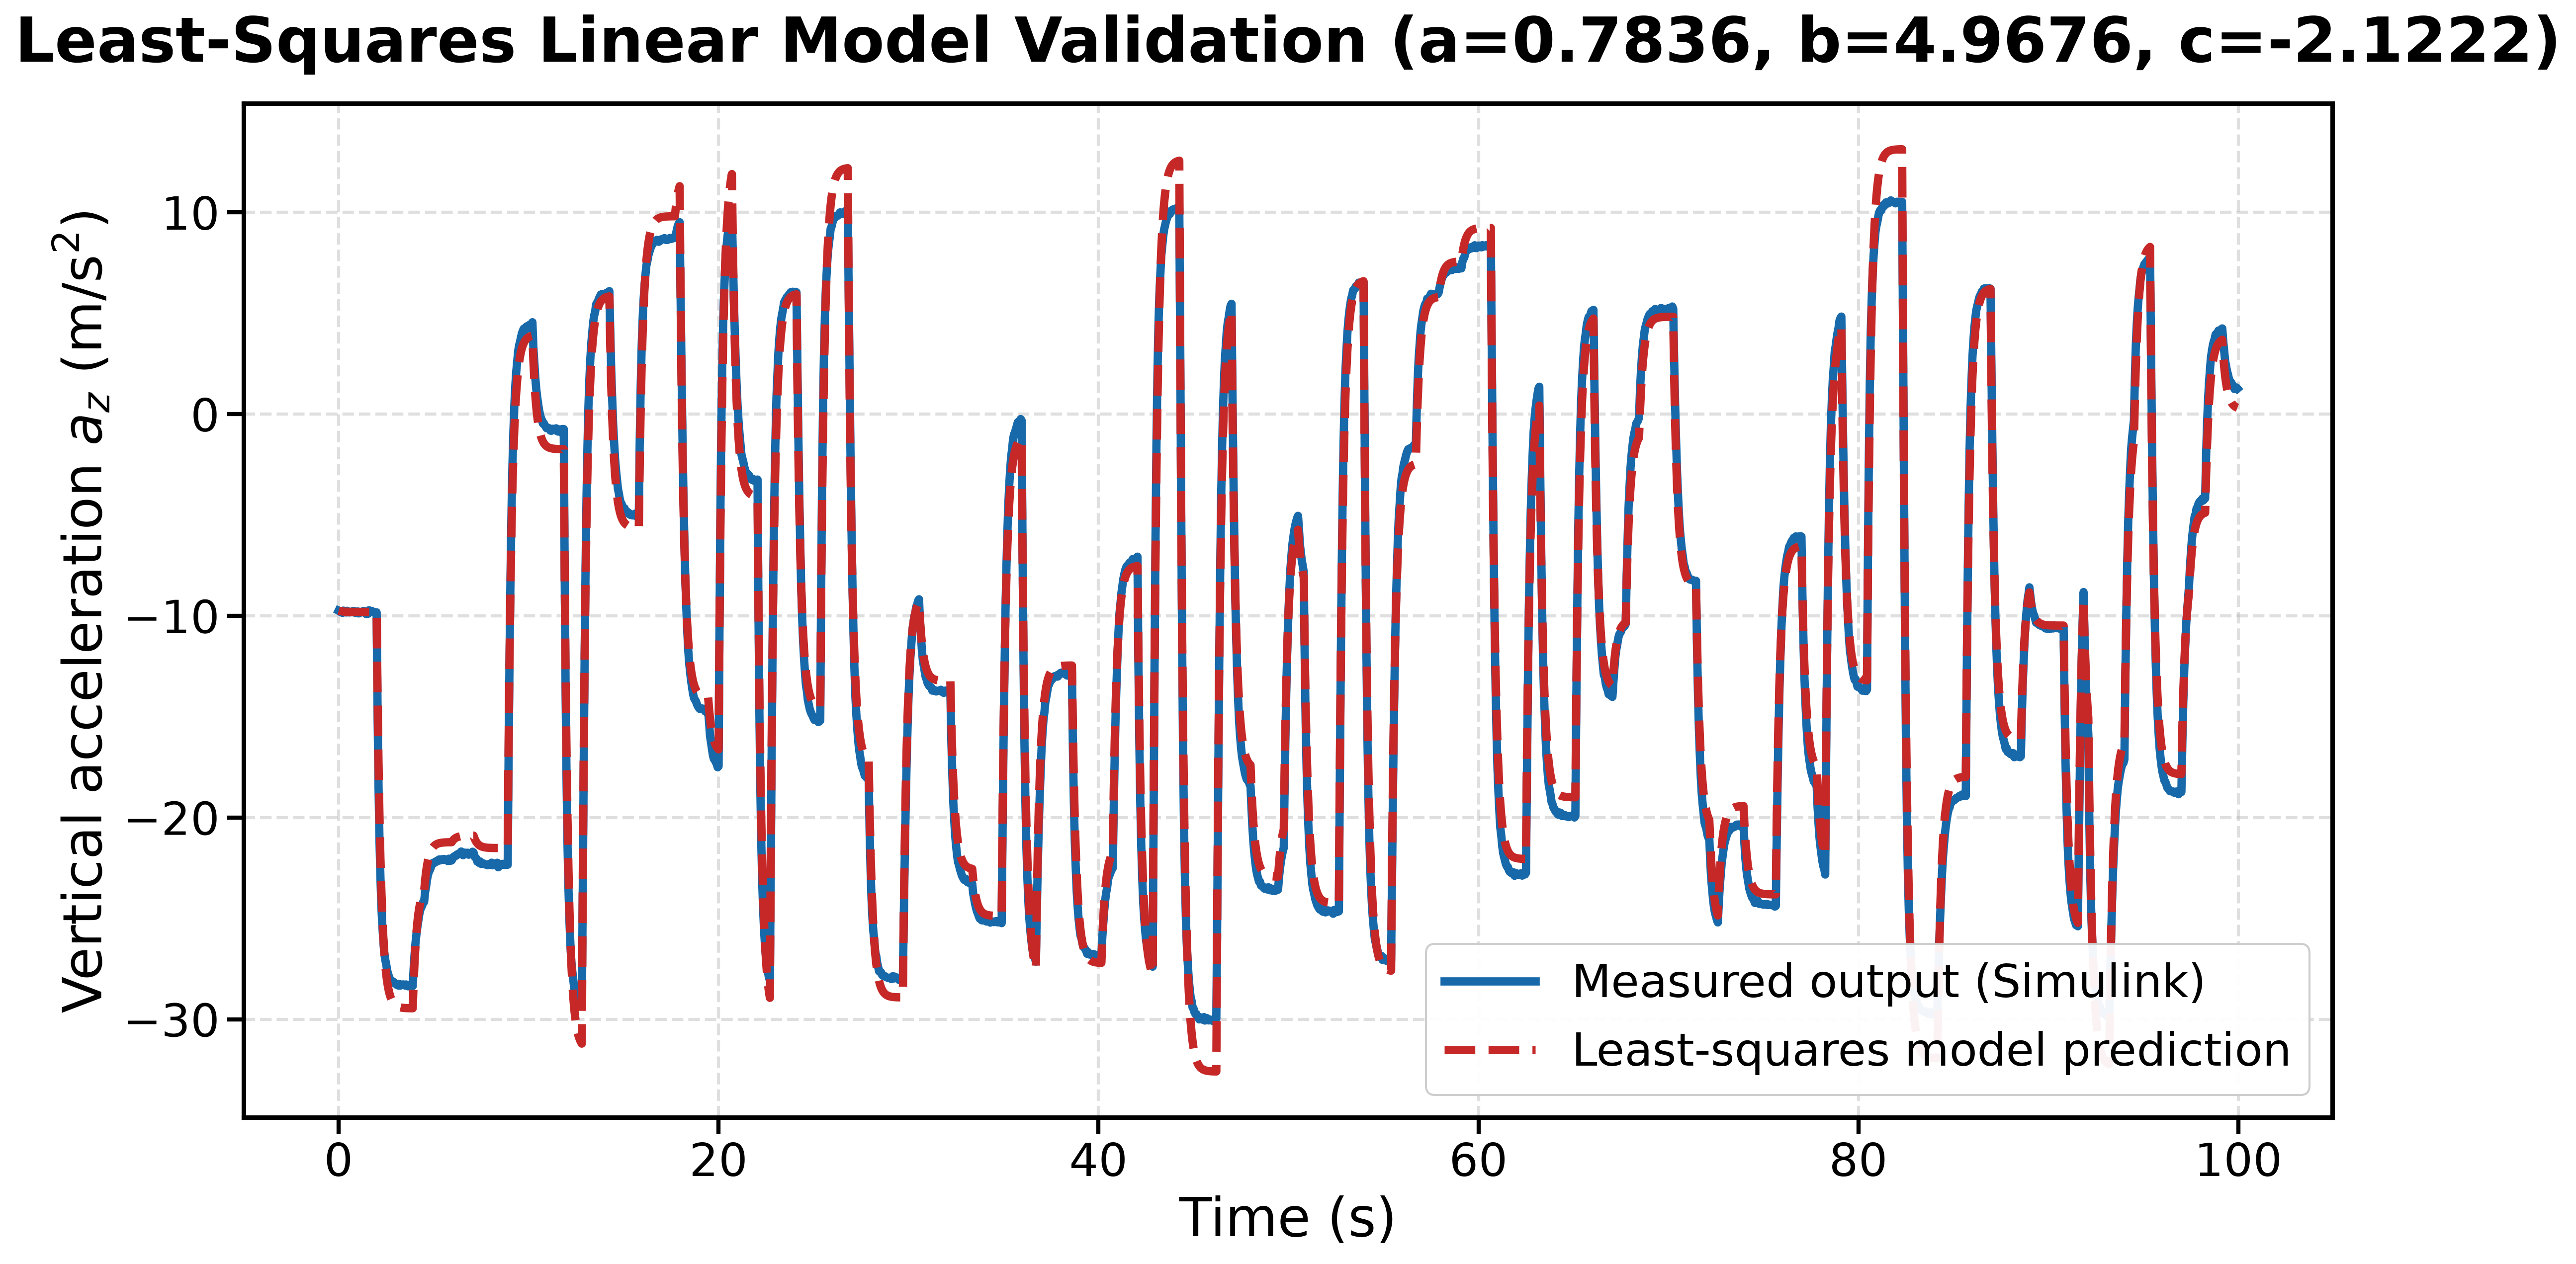
\includegraphics[
                width=\linewidth,
                height=2.75cm,
                keepaspectratio
            ]{least_squares_validation.png}
        \end{column}
    \end{columns}
\end{frame}

\begin{frame}{Appendix: System Modeling}
    \framesubtitle{Linear Model with Constant Steady-State Gain}
    \begin{columns}[T]
        \begin{column}{0.54\textwidth}
            \small
            \begin{block}{State Function}
                First-order lag driven by a constant gain $K$ and offset $c$:
                $\dot{v}(t) = \frac{1}{\tau}\bigl(K u(t) - v(t)\bigr)$,
                i.e.\ $\tau\,\dot{v} + v = K u + c$.
            \end{block}
            \begin{block}{Parameter Identification}
                - \textbf{Static gain $K$}: affine least-squares fit on steady-state regimes:
                \begin{equation*}
                    v(t) = K\,u(t) + c, \qquad K \approx 22.5,\ c \approx -9.8
                \end{equation*}
                - \textbf{Tau identification}
            \end{block}
        \end{column}

        \begin{column}{0.46\textwidth}

                \centering
                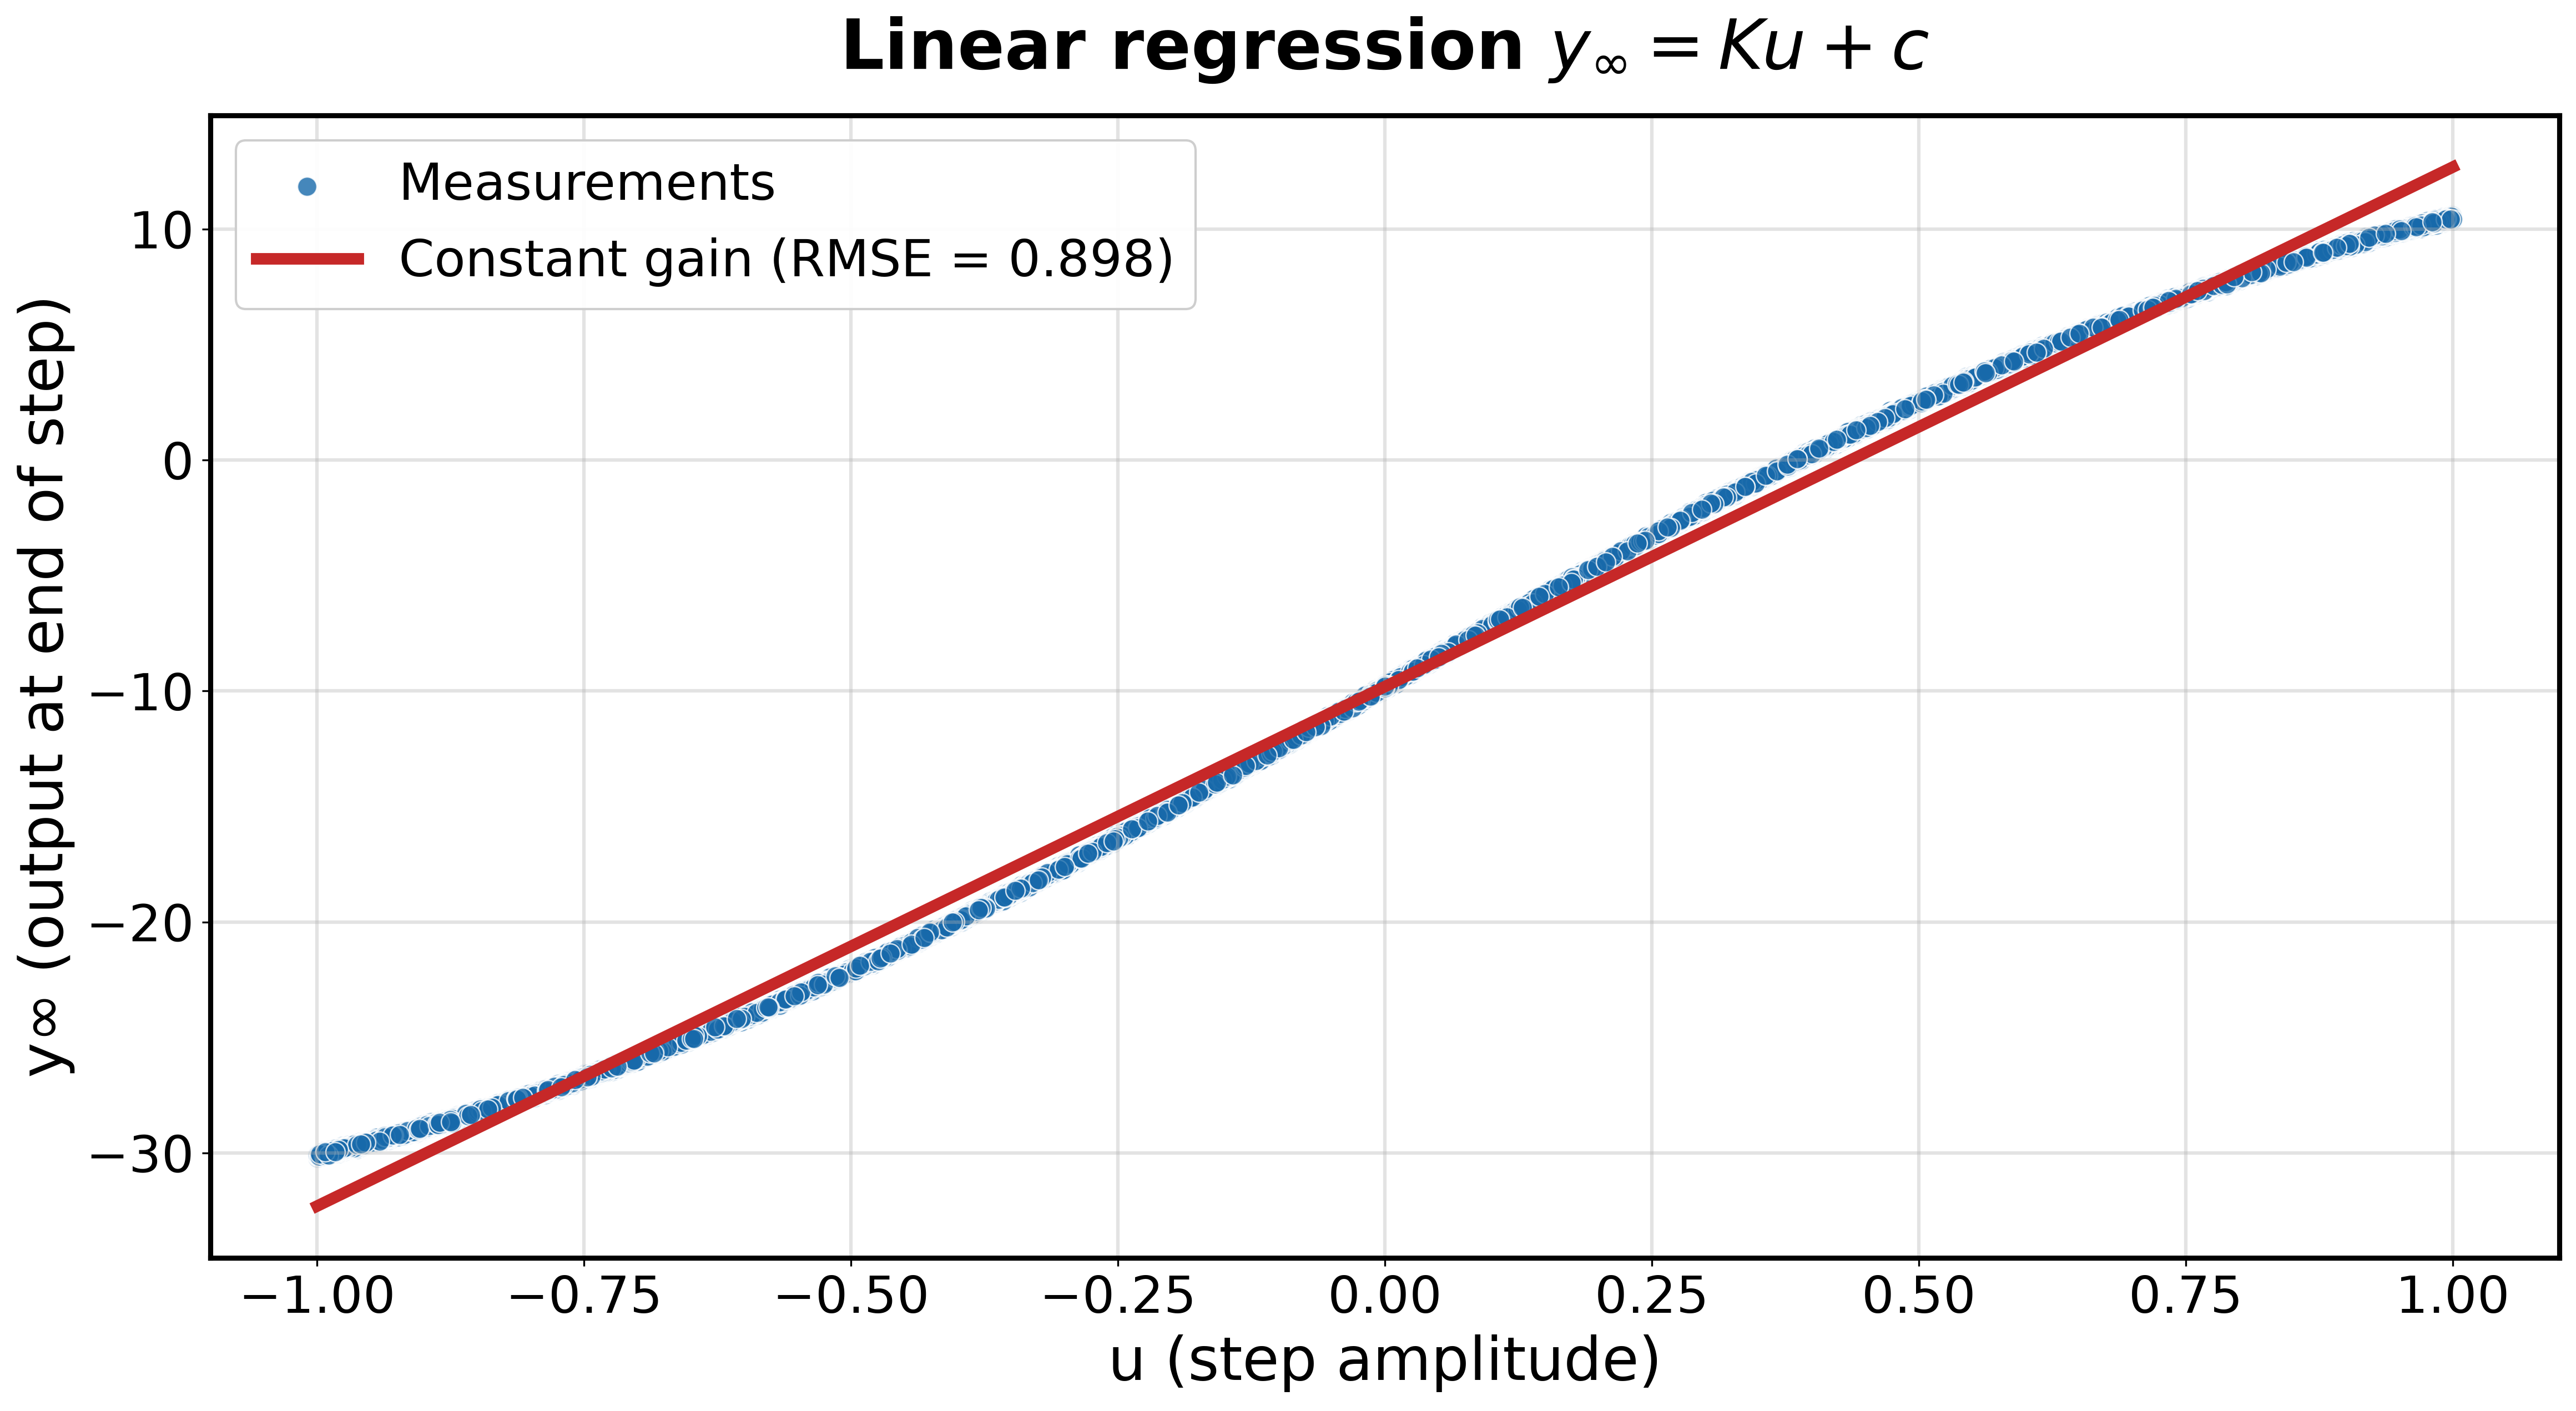
\includegraphics[
                    width=\linewidth,
                    height=2.3cm,
                    keepaspectratio
                ]{constant_gain_regression.png}


                \centering
                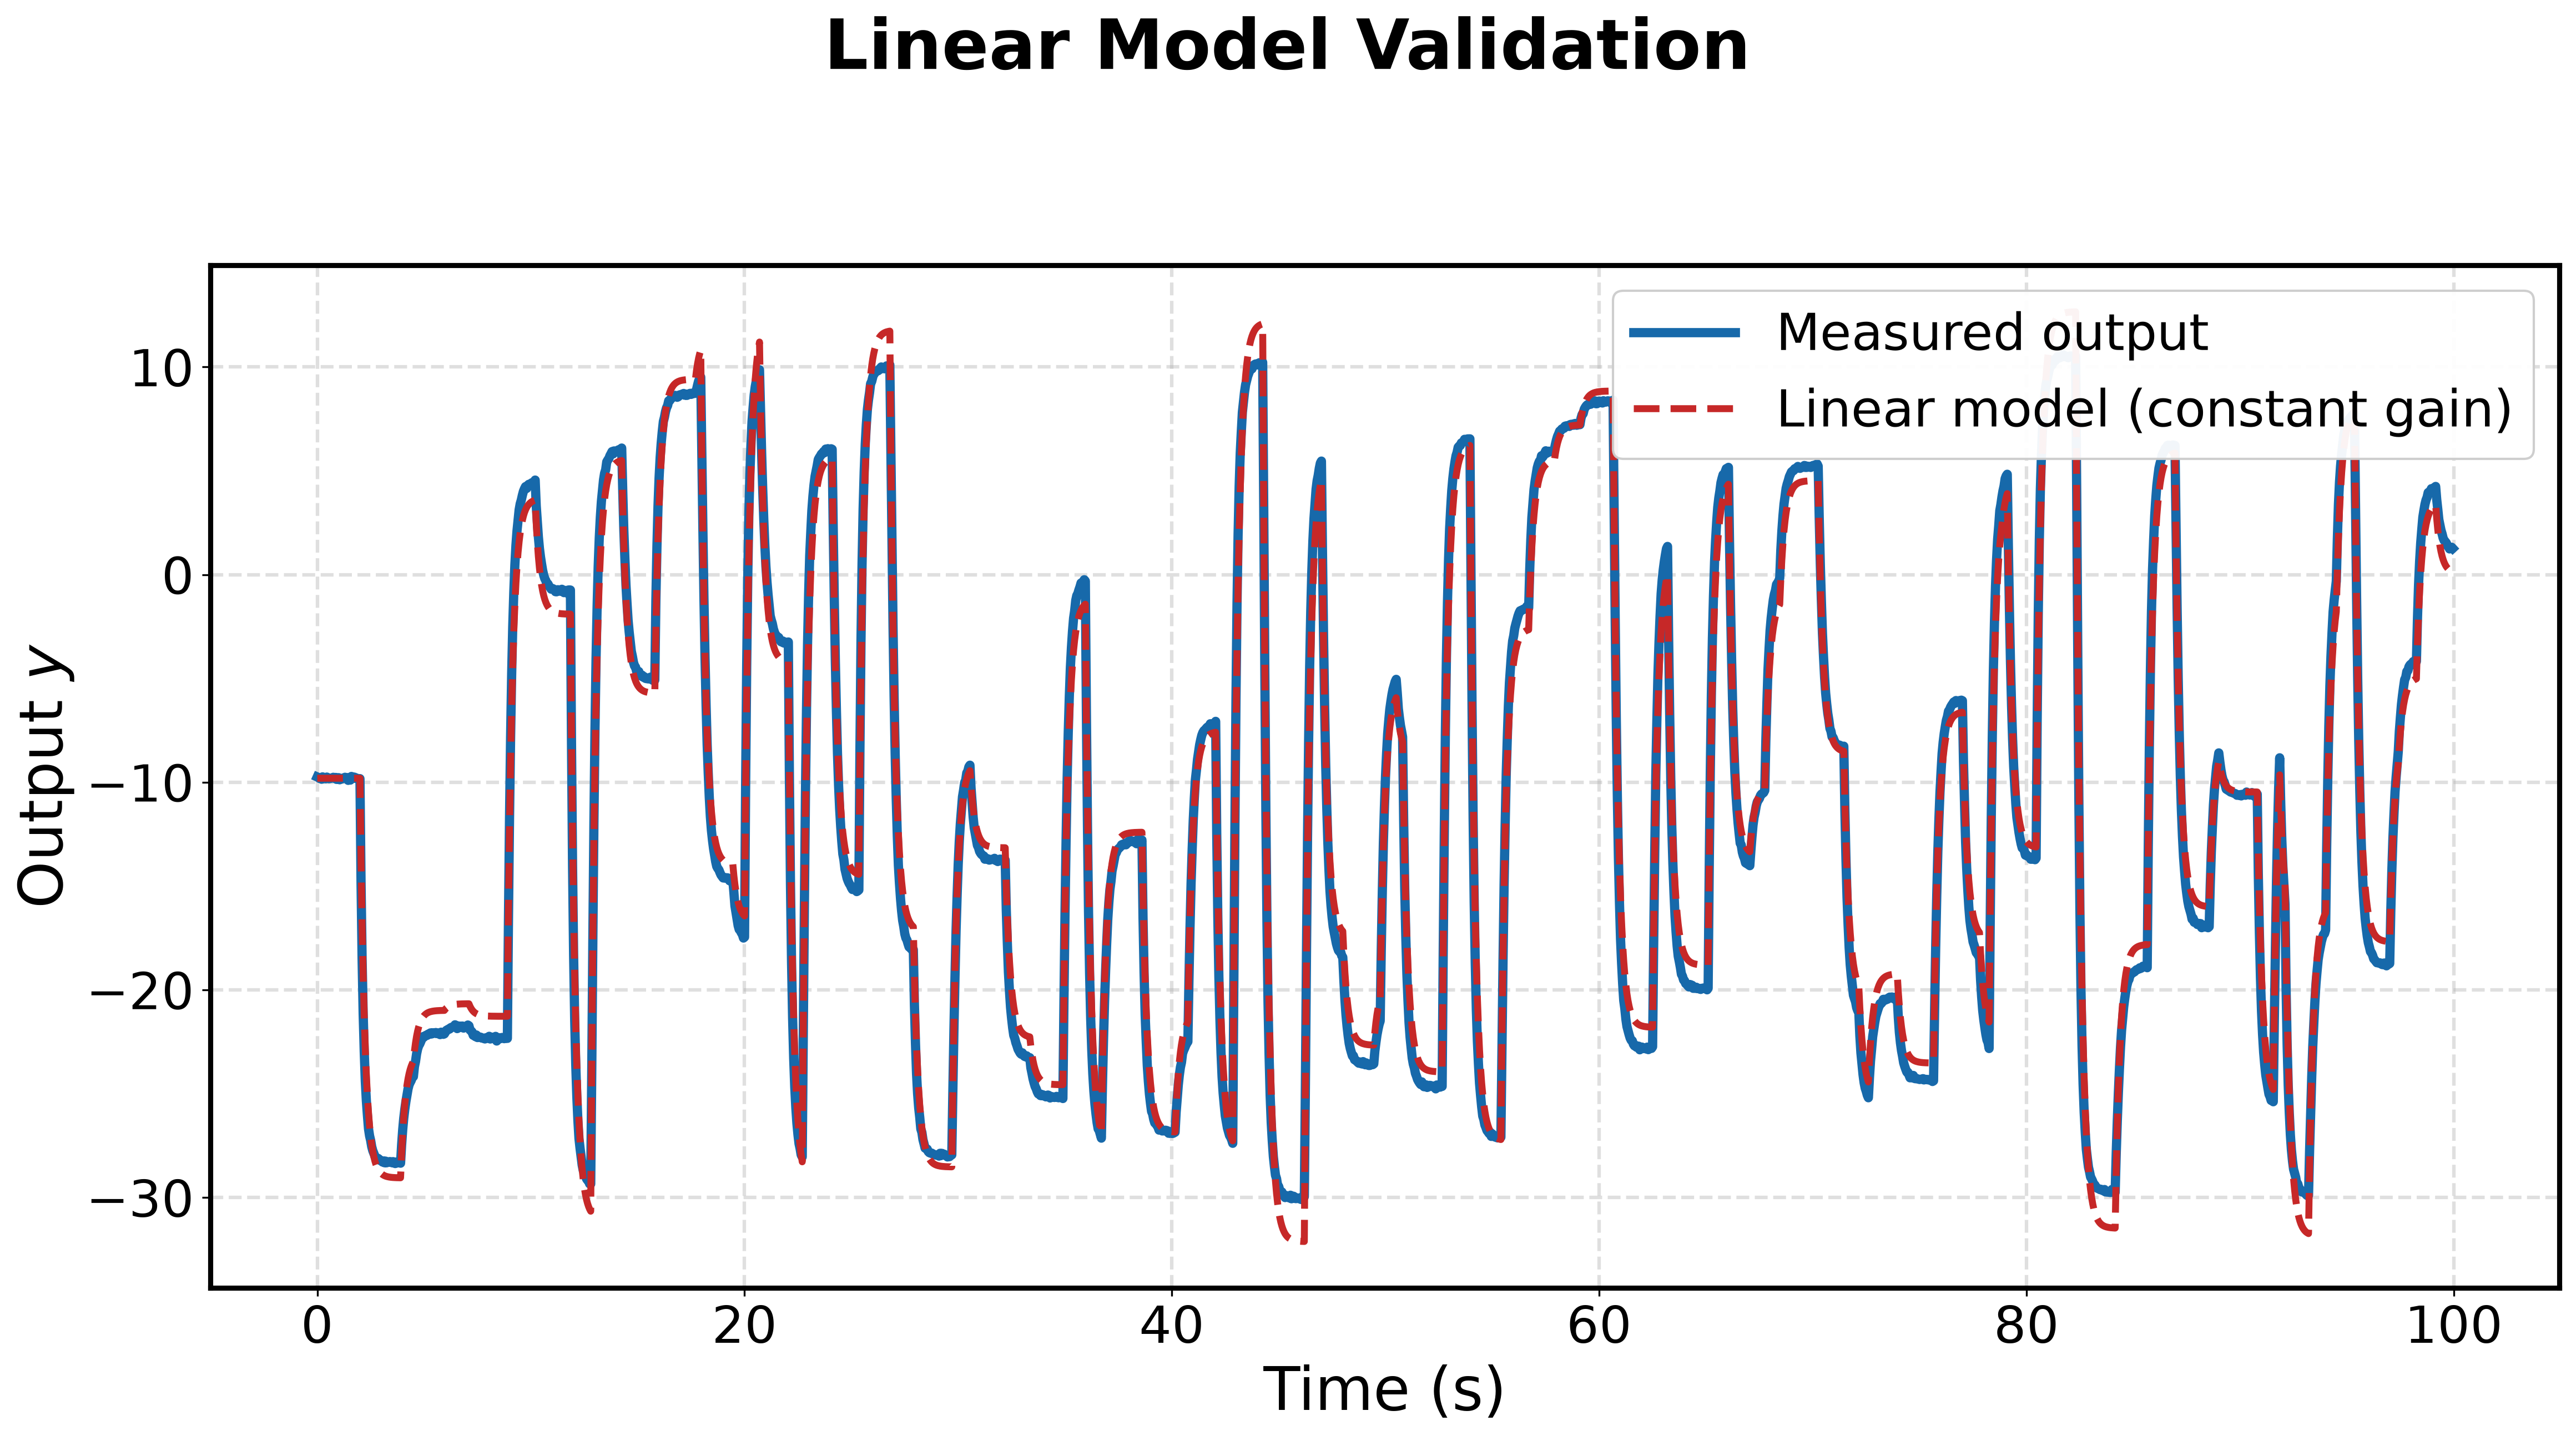
\includegraphics[
                    width=\linewidth,
                    height=6.2cm,
                    keepaspectratio
                ]{linear_gain_validation.png}
        \end{column}
    \end{columns}
\end{frame}

\begin{frame}{Appendix: Extended Kalman Filter}
    \framesubtitle{Predict and update steps}
    \begin{columns}[T,onlytextwidth]
        \begin{column}{0.48\textwidth}
            \begin{block}{Predict}
                \footnotesize
                \vspace{-6pt}
                \begin{align*}
                    \hat{x}_{k|k-1} &= f(\hat{x}_{k-1|k-1},u_{k-1})\\
                    P_{k|k-1} &= F_k P_{k-1|k-1} F_k^\top + Q,\quad F_k=\tfrac{\partial f}{\partial x}
                \end{align*}
            \end{block}
        \end{column}
        \begin{column}{0.48\textwidth}
            \begin{block}{Update}
                \footnotesize
                \vspace{-6pt}
                \begin{align*}
                    K_k &= P_{k|k-1} H^\top (H P_{k|k-1} H^\top + R)^{-1}\\
                    \hat{x}_{k|k} &= \hat{x}_{k|k-1} + K_k\,(y_k - H\hat{x}_{k|k-1} - c)\\
                    P_{k|k} &= (I-K_kH)\,P_{k|k-1}
                \end{align*}
            \end{block}
        \end{column}
    \end{columns}
\end{frame}
